\chapter{Astrophysically Triggered Searches for Gravitational Waves} % Write in your own chapter title
\label{Chapter Two}
%\lhead{Chapter~\ref{ChapterLabel}
% \emph{Astrophysically Triggered Searches for Gravitational Waves}} % Write in your own chapter title to set the page header

\section{Introduction}

Many potential sources of transient \ac{GW} signals will emit electromagnetic counterparts detectable by existing and planned astronomical instruments (see \cite{Centrella:2011nh, Metzger:2011bv, Predoi:2009af} and references therein). The coincident detection of an \ac{EM} signal would provide some of the most compelling evidence for the unambiguous direct detection of \ac{GW}, as well as provide important information on the nature of the progenitor system.

An \emph{externally triggered} \ac{GW} search represents following-up in \ac{GW} data an \ac{EM} transient, provided some information on the transient is known \emph{a priori} from astronomical observations, e.g., sky--location and time. In the next chapters I will focus mainly on the importance of analyzing \ac{GW} data around \ac{EM} events that are used as \emph{triggers} and I will describe such searches that have already been completed and others that are planned.

Searches for \ac{GW} which are \emph{triggered} by \ac{EM} observations possess several advantages over un--triggered all--sky searches. Typically, an all--sky search is performed over an entire science run, lasting months to years, and must search all sky locations for putative \ac{GW} signals. An electromagnetically--triggered search, by contrast, is usually performed over a much shorter time window lasting a few to several hundred seconds, depending on the nature of the trigger, and the sky--location of the source is usually also known to a certain degree of precision. The smaller time window increases the search sensitivity since there will be a smaller number of instrumental and terrestrial artefacts in the GW data, allowing one to identify and accept signal detections with lower significance than would be the case for a longer duration search \cite{Harry:2010fr}, see also Chapter \ref{Chapter Four}.  Knowledge of the expected time of the \ac{GW} signal allows one to make a distinction between \emph{on--} and \emph{off--source} data.  The off--source data, typically taken soon before and soon after the trigger, is used to estimate the background rate of potential gravitational wave triggers and the statistical significance of detection candidates in the on--source data, given the assumption that no GW signals from the specific EM source are to be found in the off--source (for a study of the background estimation and statistical significance of candidates see Chapter \ref{Chapter Five}). Since the noise from \ac{GW} detectors is generally non--stationary, it is important that the data used for background estimation is taken near to the trigger to accurately reflect the noise properties of the on--source data. This, however, is generally not problematic due to the fairly short on--source windows used in externally triggered analyses.  As well as the gain in sensitivity from the short on--source window, the sky--location used in electromagnetically triggered searches provides more robust signal--consistency tests in multi--detector searches and significantly reduces the parameter space of the signal, see \cite{Harry:2010fr} and Chapter \ref{Chapter Five} for a more detailed description.

Compact binary coalescence (\ac{CBC}) events are ideal source candidates for both \ac{GW} and \ac{EM} emission and the next chapters will focus on the detectability of \ac{GW} signals from \ac{CBC} events with an \ac{EM} trigger. \ac{GW} waveforms from \ac{CBC} events can be modelled theoretically and, if a detection is made, this gives an advantage over an un--modelled \ac{GW} search. By assembling a full picture of the binary parameters, using both \ac{GW} and \ac{EM} information, will lift parameter degeneracies inherent to a single \ac{GW} or \ac{EM} search \cite{Holz:2002cn, Chernoff:1993th}. Parameters such as binary luminosity distances and inclinations can be obtained from \ac{GW} search results \cite{Veitch:2009hd}. By combining \ac{GW} measurements with cosmological information, one can study the evolution of binary masses and merger rates as a function of redshift and possibly constrain merger scenarios. Second, given an associated \ac{EM} counterpart with a coalescence, it may be possible to measure both redshift and a calibration--free luminosity distance to such an event from the \ac{EM} information (spectra, dispersion measure etc.) thereby setting the energy scale and allowing an independent measurement of the Hubble constant or other cosmological parameters.

There is a series of properties that an \ac{EM} event should possess to be used as an ideal trigger for an externally triggered \ac{GW} search from a \ac{CBC} \cite{Metzger:2011bv}, namely: 
\begin{itemize}
\item
It should be detectable with present or upcoming telescope facilities -- this is necessary to ensure that systematic \ac{EM} surveys indeed take place over large times and follow--up in \ac{GW} data can be done for as many \ac{EM} events as possible, given the frequent gaps in \ac{GW} data due to poor data quality; 
\item
It should be unambiguously identifiable, such that it can be distinguished from other astrophysical transients -- this is necessary to make the association with high confidence and hence to avoid contamination from more common transient sources (e.g., supernovae, gamma--ray flares). This aspect relies heavily on the theoretical models put forward to explain the \ac{EM} transient and its origins; 
\item
it should allow for a precise determination of the sky location -- this is essential on one hand, to identifying the host galaxy and hence the redshift, as well as other relevant properties (e.g., association with specific stellar populations) and on the other hand, to minimize the sky region where the GW follow--up search will be conducted hence increasing its sensitivity. 
\end{itemize}

Short, hard gamma-ray bursts (SHB) provide a typical example of such an ideal \ac{EM} event. Constantly monitored with space--based missions, \ac{SHB} are widely believed to be the electromagnetic signatures of the coalescence of a compact binary system, consisting of two neutron stars or a neutron star--black hole and allow for a precise localization of the burst. Gamma--ray bursts have been used to trigger GW searches for some time \cite{Abbott:2007rh,Collaboration:2009kk,0264-9381-25-22-225001} and, indeed, two recent searches for GW from two \ac{SHB} whose localizations overlapped the error regions of M31 Andromeda galaxy (GRB070201, \cite{Ofek:2007th}) and M81/M82 galaxy group (GRB051103, \cite{Ofek:2006pr}) respectively, were able to confidently exclude a compact binary coalescence at the distance of M31 and M81/M82 due to the absence of significant GW emission \cite{Abbott:2007rh}. These searches did not, however, exclude a binary coalescence event at larger distances. Besides SHB, other EM transient events may play an important part in the future analyses, such as radio signatures of merging compact binaries, described in this chapter, Section \ref{section:radio}.

\section{Short Hard Gamma Ray Bursts}

Gamma-ray bursts are among the most energetic \ac{EM} phenomena in the Universe. Gamma-ray bursts were first discovered by accident at the end of the 1960's by the American Vela military mission, deployed to monitor Soviet nuclear tests. Although theories about their origin have been immediately put forward, it took almost thirty years to establish the extragalactic nature of \ac{GRB} by observing the first afterglow of a \ac{GRB} -- GRB970228 \cite{Costa:1997ji}. 

Gamma-ray bursts fall into two commonly accepted morphological groups depending on their characteristic duration of the prompt burst and spectral hardness \cite{Nakar:2007, Qinx:2010kp, Kouveliotou:1993yx, Gehrels:2006tk, Nemiroff:1993vi}, see Figure \ref{GRB_short_long}. Characteristic duration is quantitatively expressed by the $T_{90}$ parameter, defined as the time interval over which 90$\%$ of the total background--subtracted counts are observed (the total counts emitted by the source, found from the counts in the source region minus the contribution from the background), with the interval starting when 5$\%$ of the total counts have been observed \cite{McBreen:2001fd}. The majority of bursts, with softer spectrum and duration $T_{90} > \mathrm{2s.}$ are called long GRBs. They are associated with core--collapse supernova events and have been observed in optical, radio and X--ray wavelengths \cite{Campana:2006qe,Galama:1998ea,Hjorth:2003jt,Malesani:2004sg}.

\begin{figure}
\centering
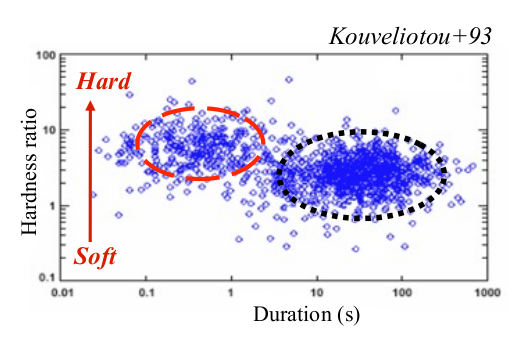
\includegraphics[scale=0.80]{Images/GRB_short_long.png}
\caption{Distribution of gamma-ray bursts in a spectrum hardness vs. duration space. The commonly--accepted ``short hard'' bursts, thought to be produced by compact binary mergers, populate the harder part of the spectrum and have shorter durations whereas the longer, softer--spectrum, unambiguously associated with stellar supernovae events, populate the lower hardness region; however, there is a region of overlap and these bursts are considered ``intermediate'' GRBs, with longer durations than SHBs, and sharing properties with the long bursts, but some with no SNe association \cite{Postigo:2010ij}. Image reproduced from \cite{Nemiroff:1993vi} for Burst And Transient Source Experiment (BATSE) bursts sample.}
\label{GRB_short_long}
\end{figure}

Those with a harder spectrum and $T_{90} \leq \mathrm{2~s}$ are labeled short hard GRBs (\ac{SHB}) and are thought to be produced by mergers of compact binaries, either binary neutron stars or neutron star-black hole. These events are ideal sources for strong gravitational wave emission \cite{ACST94, Kiuchi:2010ze}. Although the $T_{90}$ discriminator is a widely--accepted method of discerning two different classes of gamma--ray bursts, it is not a decisive indicator: e.g., recent studies have revealed the existence of an \emph{intermediate} class of \ac{GRB}, longer in duration than the typical \ac{SHB} but with the same spectral properties \cite{Veres:2010yf, Ripa:2009xs, Norris:2011tt}. It is thus important to have a full analysis of the \ac{GRB} \emph{light curves} to be able to establish its ``long'' or ``short'' nature. 

If an observation of both gamma-rays and GW originating from the same event could be achieved, it will increase confidence and allow for better science output. It is thus of great importance to constantly monitor and record SHB to allow a GW search to be performed around their burst times. Systematic analyses of GW data around short GRB times have been done in the past and the most recent publications from the LIGO--Virgo group contain results from the \emph{Swift}--observed GRBs during LIGO's fifth science run (S5) and Virgo's first science run (VSR1) \cite{Abadie:2010uf, Collaboration:2009kk} and in publication process at the time of this writing, the bursts observed by both \emph{Swift} and Fermi--GBM during S6 and VSR2 and 3, \cite{lvc:s6grb}. The analysis of the gamma--ray bursts during LIGO S6 and Virgo VSR2--3 has finished and the publication will follow soon. Another in--progress analysis effort is using GRB triggers from bursts detected by the InterPlanetary Network (IPN) and is presented in Chapters \ref{Chapter Six} and \ref{Chapter Seven}, with short--term publication plans. This effort is led by the author of this thesis.

\subsection{SHB progenitors, their host galaxies and local rates}

\paragraph{SHB progenitors}
Short GRBs ($T_{90} \leq \mathrm{2s.}$) are amongst the brightest cosmological sources of EM radiation in the Universe, with energies of $\sim~10^{48}-10^{52}$ ~erg \cite{Nakar:2007,Berger:2010qx}. Given the short duration and spectral hardness, their progenitors are widely believed to be mergers of \emph{compact} objects, either neutron star--neutron star (NS--NS) or neutron star--black hole (NS--BH) binaries \cite{Paczynski:1986px, Nakar:2007, Belczynski:2006br, Troja:2007kt, Metzger:2011bv, Capozziello:2010sm, Berger:2010qx} (and references therein). There is no conclusive observational evidence supporting this case, therefore in the next paragraphs we will mainly list a series of short hard GRB properties that differentiate them from the long soft GRB population, in an indirect way of motivating a compact binary merger progenitor model for them.

A good indicator of their progenitor would be securing a host galaxy for each burst, preferably with very low or extinct star formation, the most likely host for compact binary mergers formed at the peak of the galactic star forming period \cite{Kelley:2010qx}. A host galaxy can be identified by observing an \ac{SHB} afterglow, localized to sub--arcsecond precision; usually, an X-ray afterglow is observed first, that will trigger an optical follow--up with results of sub--arcsecond precisions. Although some \ac{SHB} afterglows have been observed in different wavelengths, short hard GRBs are known for weak afterglows, making it difficult to obtain a large enough sample for unambiguous statements. Prior to 2005, when the first optical and X-ray afterglows of SHB were detected, the compact binary progenitor model had been a viable theoretical explanation of the energetics and emission mechanism of such bursts with no observational support. After the first afterglows of SHB have been detected (e.g., GRB050509B, GRB050709 and GRB050724, \cite{Pedersen:2005kh, Nakar:2007xe}), a few important observations have been made to partially support the compact binary merger progenitor model and partially to prove that the SHB origins differ from long GRB's. First, their X-ray and optical afterglow spectra could not be associated with core--collapse supernovae (the observationally confirmed progenitor of long GRB \cite{Woosley:2006fn}). Second, based on afterglow observations, most of the hosts are identified to be star--forming galaxies (ratio 4:1 to old galaxies \cite{Berger:2010qx}) but with lower star formation rate (SFR) and higher metallicity than the hosts of long bursts \cite{Berger:2010qx}; a few hosts have been identified as old elliptical with almost null SFR. 

For the few SHB that have confirmed redshifts to date, their redshift distribution is inconsistent with a bursting rate that traces the SFR in the universe, unlike long--soft GRBs, which do follow it \cite{Prochaska:2005qf}. The association with low(er)--SFR galaxies and their position within these galaxies support an old ($\sim$~Gyr) progenitor, like NS--NS or NS--BH binaries.

Another argument in support of the compact binary coalescence progenitor model for \ac{SHB} is the redshift--luminosity two--dimensional distribution \cite{Nakar:2007}. The SFR is higher at larger redshifts ($z \geq 1$) and a lot of the \ac{SHB} are observed at lower redshifts ($z \geq 0.3$) -- this implies that the progenitors are born when the Universe is still young and produce the \ac{SHB} at a much later stage, explaining time differences of $\sim$Gyr, hence old compact binaries.

One recent proposal put forward to distinguish short hard from long soft--spectrum bursts is the still controversial so--called ``Amati relation'' between the peak energy in gamma-rays ($E_p$) and the isotropic equivalent radiated energy ($E_{\gamma, \mathrm{ISO}}$) for bursts with known redshift \cite{Amati:2002ny}. This empirical relation states that $E_p \propto E_{\gamma, \mathrm{ISO}}^{0.5}$ for long soft bursts and the short bursts do not follow this proportionality relation (are outliers). There is, however, a wide spread in the data distribution and the instrumental effects are still unclear, to identify this as a definitive argument in differentiating short from long bursts.

Consider now that we accept the compact binary merger progenitor model for SHB; we would want to differentiate the binary NS or the NS--BH types of mergers. Due to a relatively small number of SHB afterglow observations, and if SHB are truly compact binary merger events, it is still unclear what proportion of the bursts are produced by either NS--NS or NS--BH mergers. A few models have been put forward trying to relate the progenitor nature with its environment.

Based on burst durations and X-ray afterglow extended emission, measured redshifts and locations for a sample of SHB, according to \cite{Troja:2007kt}, SHB with measured offsets from host galaxies appear qualitatively divided into two groups. The group with larger $T_{90}$ durations and afterglow extended emission all lie very close to their hosts, favoring an NS--BH merger progenitor (this, supported by two arguments: the BH might not have received an energetic ``kick'' at its birth \cite{Mirabel:2003st} and the merger times for NS--BH systems are of order 100 shorter for a $1.4 - 14 M_{\odot}$ system), while the group with shorter durations and no extended emission have a mean offset of factor $\sim$~15 larger, favoring an NS--NS merger as progenitor. 

There is also variety in characteristic ages of the binaries that are thought to produce the SHB -- reference \cite{Belczynski:2006br}, based on the known Galactic binary pulsars and using a population synthesis model, infers that there are two classes of binaries -- ones with old ages of $\sim$~0.1-15 Gyr before merging (80$\%$ chances to be NS--BH) and others with much shorter ages of $\sim$~0.001--0.2 Myr (equally probable to be NS--NS and NS--BH). This leads to a possible association with host galaxies: for starburst galaxies (which on average have small masses) where stellar populations are young, mergers from short--lived double compact objects are expected; in elliptical galaxies, with a very low SFR, mergers of long--lived double compact objects are expected.

Although binary coalescence is the favored progenitor model for short GRBs, this has not yet been confirmed by means of a direct observation and some other progenitor models have been put forward as alternatives, for instance reference  \cite{MNR:MNR12923} proposes that SHB may originate from double white dwarf mergers. Consequently, the detection of gravitational waves associated with a short GRB would provide evidence that the progenitor is indeed a coalescing compact binary and also provide information on the parameters of the binary (most importantly the masses for NS--NS and masses and spins for the NS--BH case).

\paragraph{Binary merger rates}
\label{shbrates}
Unfortunately, actual observational constraints on compact binary populations may be obtained only for NS--NS systems since only such binaries are currently directly observed as binary pulsars (e.g., the three known systems: Hulse-Taylor PSR B1913+16, B1534+12, and J0737-3039 \cite{Kim:2006fm}, also described in Chapter \ref{Chapter One}). Merger rates extrapolated from the observed sample of Galactic relativistic NS--NS binaries have been presented in \cite{Nutzman:2004bw,Kim:2006fm} (and references therein). 

Based on the number of galactic binary pulsars, according to \cite{Nutzman:2004bw} the best estimate of the NS--NS merger rate in the Galaxy is presently $\sim 10^{-5}-3 \times 10^{-3}~\mathrm{yr}^{-1}$. All extrapolations from Galactic to extragalactic rates are based on the assumption that the formation of binary compact objects in a region is proportional to the blue luminosity in that region, corrected for reddening \cite{Phinney:1991ei}. Based on this, the rates convert to $\sim 2 \times 10^2-3 \times 10^3~\mathrm{Gpc}^{-3}\mathrm{yr}^{-1}$ for a galaxy number density of $10^{-2}~\mathrm {Mpc}^{-3}$. This would imply a LIGO/Virgo rate of $\sim 5 \times 10^{-3}-0.1  ~\mathrm{yr}^{-1}$ for the present detectors. More recently, and again based on the known binary pulsars, according to \cite{Kim:2006fm}, the NS--NS merger rate within the Galaxy should be in the range $\sim ~10^{-6}-1.5 \times 10^{-4} ~\mathrm{yr}^{-1}$ implying LIGO/Virgo event rates in the range $\sim ~4 \times 10^{-4}-6 \times 10^{-2} ~\mathrm{yr}^{-1}$ for the present detectors and $\sim ~2-330 ~\mathrm{yr}^{-1}$ for the advanced detectors.

In \cite{Nakar:2007} the range for the volume rates for short hard GRBs considered compact binary mergers, at redshift null and detectable with present gamma-ray telescopes are estimated to $\sim ~10-10^4 ~\mathrm{Gpc}^{-3}\mathrm{yr}^{-1}$ which would imply a detection rate of $7 \times 10^{-4} - 7 \times 10^{-1} ~\mathrm{yr}^{-1}$ for the present LIGO/Virgo, assuming a naive uniform volume distribution of SHB events (justified by an isotropic distribution of long and short bursts, observed by BATSE). These rates are consistent with the expected binary neutron star merger rates.

\subsection{Emission mechanism}
\label{SHBmodel}

The coalescence of a compact stellar-mass binary (either two neutron stars or a neutron star and a black hole companion) is the endpoint of its (presumed) $\sim$ Gyr life revolving around the common center of mass while constantly losing energy and angular momentum through emission of gravitational radiation. The binary merger will lead to the formation of either a transient hyper-massive highly magnetized neutron star with a lifetime of a few ms \cite{Shibata:2005mz, Duez:2005cj} that will collapse to a rapidly spinning black hole or straight to the formation of a black hole \cite{ShibTan06, Shibata:2007zm}. In the favored model of short GRBs \cite{Shibata:2005mz, Kiuchi:2010ze, Rezzolla:2011da, Oechslin:2005mw}, the gamma-ray emission is contingent on the formation of a massive (and highly magnetized) torus around the final black hole. The matter in the torus is accelerated to relativistic velocities leading to the formation of a collimated jet of electromagnetic radiation along the axis of the former binary total angular momentum. Differences in velocities between layers in the jet account for the prompt gamma-ray emission.

\paragraph{GW--gamma-ray emission time difference}
A critical parameter in searching for GW associated with SHB is the difference in the burst/GW arrival times at the Earth. Several semianalytical calculations of the final stages of a NS--BH inspiral show that the majority of matter plunges onto the BH within order 1s \cite{Davies:2005}. Full relativistic and magnetohydrodynamic numerical simulations have shown that the time difference between the binary merger and the jet formation can be between a few milliseconds up to a few seconds \cite{ShibTan06, Shibata:2007zm, Rezzolla:2011da, Rezzolla:2010fd, Baiotti:2008ra, Oechslin:2005mw}.

\begin{figure}
\centering
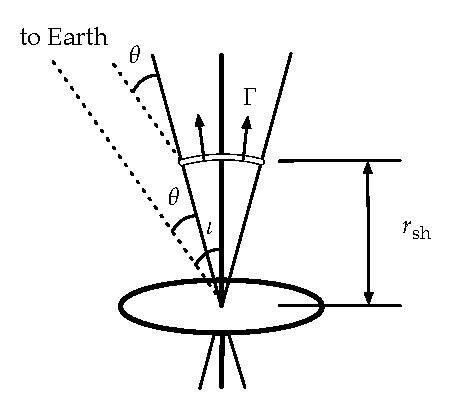
\includegraphics{Images/CBC_geometry}
\caption[Geometry of the compact binary coalescence model of short GRBs]
{Geometry of the compact binary coalescence model for short hard gamma-ray bursts.
Parameters are: $r_\mathrm{sh}$ is the distance between the central engine and the inner
shock, $\iota$ is the inclination angle, which is the angle between the
line of sight of an Earth--based observer and the orbital axis.
Although we generally believe that Earth is within the jet opening angle,
we depict the angle $\theta$ between our line of sight with the engine
and our line of sight with the nearest outflow direction for generality. This choice of angles makes the distinction between the outflow half--opening angle (the jet angle, $\iota - \theta$) and the observed inclination angle -- there might be the case that a GRB is observed after a jet break. In the cases we will follow further on, we will assume that the observer is placed within the jet cone, reducing to $\theta=0$. Image first published and reproduced from \cite{NickThesis}.}
\label{fig:internal_shock_geometry}
\end{figure}

The jet outflow will be characterized by a Lorentz factor $\Gamma \gg 1$ with a variability of order $\Gamma$. A secondary outflow with Lorentz factor $2 \times \Gamma$ will impact the first outflow at a distance $r_\mathrm{sh}$ after $\delta t_\mathrm{engine}$ s. Given an observer at infinity at rest with respect to the central engine, $r_\mathrm{sh} \approx \frac{8}{3} c \delta t_\mathrm{engine} \Gamma^2$ \cite{NickThesis}, where $v$ is the velocity corresponding to $\Gamma$. Assuming that gravitational waves propagate at the speed of light in vacuum, the delay between the GW and the $\gamma$-ray signals will be the path difference, as in Figure \ref{fig:internal_shock_geometry}. With this na\"ive picture, the total time delay observed at Earth will be
%
\begin{align}
\label{eq:time_delay}
  \delta t_\mathrm{GW-EM}
      &=  \frac{r_\mathrm{sh}}{v} - \frac{r_\mathrm{sh}}{c} \cos \theta
          \nonumber\\
      &=  \frac{8}{3} \delta t_\mathrm{engine} \Gamma^2
          \left(1 - \cos \theta\right) \,,
\end{align}

\noindent where $\theta$ is the angle between the observer's line of sight to the central engine and the observer's line of sight to the internal shock. Note that $\theta$ is different from the binary inclination angle $\iota$, which is the angle between the observer's line of sight and the orbital angular momentum vector. This choice of angles makes the distinction between the outflow half--opening angle (the jet angle, $\iota - \theta$) and the observed inclination angle -- there might be the case that a GRB is observed after a jet break. In the cases we will follow further on, we will assume that the observer is placed within the jet cone, reducing to $\theta=0$. The central engine's dynamical timescale is between the light-crossing time of the final BH and the plunge time of the NS matter, so we take $t_\mathrm{engine} \approx 10~\mathrm{ms}$. Short GRBs have Lorentz factors $\Gamma$ measured to be in the range $10$--$50$ \cite{NakarReview:2007}. To receive a substantial gamma-ray flux at Earth, it is reasonable to assume that we are within the jet opening angle. Setting $\theta = 0$ gives $\delta t_\mathrm{GW-EM} = 0~\textrm{ms}$. At maximum, we must be within $\theta \approx 1 / \Gamma$ of the shock front, which gives $\delta t_\mathrm{GW-EM} \approx 40~\textrm{ms}$. We exclude the interstellar and intergalactic media as contributing to time delays, as the index of refraction at these energies (1$\mathrm{MeV} = 2.4 \times 10^{20}~\mathrm{Hz}$) is negligible.

Therefore, supposing gravitational waves produced just before merger travel at the same speed as the gamma-rays, the speed of light in vacuum, and suppose the observer is situated within the cone of the jet, one would expect to observe the GW within one to a few seconds prior to the arrival of the gamma rays. As the GWs emitted during the pre-merger inspiral dominate the signal-to-noise-ratio (SNR) observable in current GW detector data and they can be accurately modelled using Post-Newtonian approximations \cite{ABIQ04, AIQS06a}, our searches will be aimed at this phase only.

\paragraph{Are short gamma-ray bursts collimated?}
Unlike other high--energy astrophysical phenomena e.g., Active Galactic Nuclei (AGN) or galactic micro--quasars, gamma-ray burst images are poorly resolved and the structure of the outflow can only be indirectly estimated from observations of the afterglow properties \cite{Granot:2010iq}. Although they are believed to be collimated, the evidence for jets (i.e., highly collimated outflows) in GRBs is mainly indirect. There are several implicit arguments that support a collimated emission from GRBs: 

\begin{itemize}
\item
Other highly relativistic outflow sources (AGN, micro--quasars) are collimated and if the GRB emission mechanism is indeed similar to those (accretion onto a black hole) then it would be only natural that GRBs are collimated too; 
\item
Very high values of $E_{\gamma, \mathrm{ISO}}$ can be explained only if the emission was collimated -- if the outflow is collimated into a narrow jet that occupies a small fraction of the total solid angle, then the strong relativistic beaming due to the very high initial Lorentz factor ($\Gamma_0 > 100$) will cause the emitted gamma rays to be similarly collimated; if it was a close to spherical explosion, ejecta with such high Lorentz factors would carry away only a small amount of energy, insufficient to account for very high values of $E_{\gamma, \mathrm{ISO}}$;
\item
A more direct explanation for collimation would be by observing a ``jet--break'' in the GRB afterglow: due to relativistic beaming, most of the observed emission comes from a visible region of angle $\sim1/\Gamma$ around our line of sight; as the outflow advances in the surrounding medium, consequently decelerating, the jet widens to the point where the observer would ``miss'' the flux from outside the jet edge (i.e., a jet break). This would have been present if the flow were spherical, resulting in a faster flux decay. The beaming factor, given a jet that is uniform within its half--opening angle $\theta_0$, is $f_b=1-\cos \theta_0$ and for derived values of $f_b \approx 10^{-3}~-~10^{-2}$, jet half--opening angles would range from a few degrees to a few tens of degrees \cite{Granot:2010iq}. The only short GRB for which a jet--break was observed in the afterglow is GRB051221A with an initial opening angle $\sim$4--8 degrees \cite{Burrows:2006ar}.
\end{itemize}

Given the model--dependent assumptions and the few astrophysical observations to--date limiting the jet--opening angles for short GRBs, it is not yet clear if they are highly collimated or not. However, there is no indication as of yet, that the emission is within a large opening angle or spherical either. Considering the case that the GRB observation is made within the emission cone (i.e., setting $\theta = 0$, inclination angle $\iota$ is identical to the jet half--opening angle), it is useful to understand what range of inclination angles $\iota$ we would expect from an observed short gamma-ray burst; this information is not only important from the pure GRB observational point of view, but, as we will see in Chapter \ref{Chapter Four} and Chapter \ref{Chapter Six}, will be important in GW searches associated with short GRBs. As such, we will consider that short GRBs are mildly collimated with half jet--opening angles no larger than 45 degrees.  

\subsection{Gamma ray observation missions}
There has been a series of space-based missions surveying the gamma-ray skies since the early 1960's. The first dedicated GRB satellite was the Compton Gamma-Ray Observatory (CGRO) launched by NASA in 1991 (together with its on--board high energy detector Burst And Transient Source Experiment or BATSE). Although de-commissioned in 2000, data from CGRO was extensive and is still analyzed even today. Nowadays, the three most important GRB detectors are \emph{Swift}, Fermi--GBM and the InterPlanetary Network (IPN), summarized below.

\paragraph{\emph{Swift}:}
\emph{Swift} \cite{swiftdatasheet} is an international mission operated by NASA Goddard Flight Center, launched in November 2004 and placed in near--Earth orbit. It consists of three telescopes operating in different wavelengths: the Burst Alert Telescope (BAT), a gamma-ray telescope with very good angular resolution (1 to 4 arcminutes), the \emph{Swift} X-ray telescope (XRT) and ultra--violet telescope (UVOT) responsible for burst position refinement and identification of afterglows. When a GRB occurs, the BAT will be the first of \emph{Swift}'s instruments to observe it; within about 10 seconds of the burst trigger, the BAT produces a burst localization, which is transmitted to ground observers. In addition, the BAT's position is fed to the \emph{Swift} spacecraft so a slew can be performed, bringing the GRB into the XRT (3--5 arcseconds location accuracy) and UVOT's (0.3 arcseconds location accuracy) fields--of--view. The BAT continues to record counts that will produce the gamma-ray light curve while both the XRT and the UVOT will transmit afterglow light curves after 20 minutes and 2 hours, respectively.  

\paragraph{Fermi--GBM:}
\emph{Fermi/GBM} (formerly known as Gamma-ray Large Area Space Telescope or GLAST \cite{fermisite2}) is a multi--national mission launched in 2008 in near--Earth orbit and operating two on--board gamma-ray detectors: the Large Area Telescope (LAT), a highly advanced telescope with an approximate field--of--view of 20\% of the sky and a very high energy threshold (order $\sim$ 300 GeV) and the gamma-ray Large Area Telescope (LAT) with a broad field--of--view (2/3 of the sky) but less powerful in terms of energetics and burst localization.

\paragraph{The InterPlanetary Network:}
The InterPlanetary Network (IPN) \cite{Hurley:2002wv, Hurley:1999ym} employs several space missions and synthesizes data obtained from the detection of the same burst by different spacecraft equipped with gamma-ray detectors. The IPN has been operating for three successive generations; presently the third IPN (IPN3) began its operation in November 1990. Currently the spacecraft gathering data are Konus-WIND, Suzaku--WAM, INTEGRAL,  RHESSI, \emph{Swift}, Fermi--GBM, AGILE (in Earth orbit), MESSENGER (in Mercury orbit) and Mars Odyssey (in Mars orbit) \cite{HurleyHTML}. When the duty cycles and effective fields of view of all the missions in the network are considered, the IPN is close to being an all--time, isotropic GRB monitor. 

The minimum number of IPN spacecraft observing a burst is two since the operational principle for IPN GRB detections is triangulation using different burst times of arrival at different spacecraft. The larger the distance between satellites (``baseline''), the better the localization accuracy. This will be described in detail in Chapters \ref{Chapter Six} and \ref{Chapter Seven}, where we will present the method and analysis results of the search for GW associated with the IPN--detected short bursts during S5/VSR1. The IPN, given that most of the participating missions are wide--field telescopes, has a wide range of spatial sensitivity. This depends on the relative positions of the available spacecraft observing a certain burst. Burst localization is made to error regions ranging from fractions of square degrees to hundreds or thousands of square degrees. Of the IPN missions, \emph{Swift}, Fermi--GBM, INTEGRAL, and AGILE have the capability of following--up an initial relatively poorly localized GRB detection with onboard imaging telescopes, allowing refined sky localization and an observation of light curves and afterglows.

Some GRB events may be observed coincidentally by both Fermi (the GBM) and the IPN and the resulting combination of sky positions may reduce the overall error region.

\paragraph{Future missions:}
With the previewed retirement of \emph{Swift} in the next years (no earlier than 2015), it is very important to find out if there is continuation of momentum in the field of observational gamma-ray astronomy. One of the future missions, the Space--based multi--band astronomical Variable Object Monitor (SVOM), a Chinese--French collaboration mission \cite{Schanne:2010fu} set to be launched in 2016, is anticipated to take \emph{Swift}'s role. Operating a set of four detectors, including a powerful visible telescope (VT), the SVOM will see an estimated 75$\%$ of all the GRBs and will be able to identify, with minimal delays, their X-ray, optical and UV afterglows. In addition to SVOM, both Fermi--GBM and the IPN will be operational beyond 2015, albeit a few of the IPN missions will be decommissioned.   

\subsection{Astrophysics with SHB and GW}
\label{importanceGWSHB}
Simultaneous detection of the inspiral GW signal from a compact merger and a SHB will provide conclusive evidence that SHBs originate from compact mergers and would improve our understanding of both merger physics and SHBs significantly. 

Information on binary component masses, spins and equation of state of the NS \cite{Kyutoku:2011vz} can be extracted from the GW signal, parameters that are impossible to be determined solely from the gamma-ray observations; general relativity can be tested in the strong field regime \cite{lrr-2006-3}. Coincident detections of GW and SHB may be used, in the next generation GW detectors' era, to constrain cosmological parameters (the Hubble constant) \cite{Dalal:2006qt}; GW detections will provide a measure for a calibration--free distance to the burst while possible observations of electromagnetic afterglows will provide us with a measure of the redshift, this way using SHB events as "standard sirens" for cosmological parameters' measurements.

Depending on the central engine evolution, the beaming of an SHB prompt emission may differ from that of the lower energy \emph{orphan} afterglow; observations of the afterglow may not be preceded by gamma-ray detections \cite{Nakar:2002un} but may still be used in a delayed coincidence with GW detections. However, orphan afterglows should be searched for quickly, within days or weeks after the GW detection since the GW detection will have originated from a nearby SHB (distance $<$ 500 Mpc) and given that the less energetic SHB are more numerous, chances are that the orphan afterglow will not last a long time. The beaming angle can be constrained from GW observations: the binary inclination angle parameter enters the GW waveform and can be recovered. We will see in Chapters \ref{Chapter Five} and \ref{Chapter Seven} how gravitational wave searches can constrain its value. Once this is known for an orphan afterglow, it could be established if the burst was indeed beamed and observed off--axis hence no gamma-ray observations or was on--axis and not beamed.

Several searches for gravitational waves associated with gamma-ray bursts have been performed in the past using data from both LIGO and Virgo detectors \cite{abbottgrb05,burstGrbS234,Ac_etal:07,Ac_etal:08}. Most recently, data from the sixth LIGO science run (S6) and the second and third Virgo science runs (VSR2 and 3) were analyzed to search for \ac{CBC} signals and unmodelled gravitational wave bursts (GWBs) associated with both short and long GRBs from 2009--2010 \cite{lvc:s6grb}. Although long GRBs are not expected to be produced after a compact binary merger event, an opportunistic search around long GRBs times was still performed. No evidence for a \ac{GW} signal was found in these searches. Additionally, two in--depth analysis papers, analyzing GRB~051103 and GRB~070201 were published \cite{Abadie:2012bz} and \cite{Abbott:2007rh}, respectively. These two short-duration GRBs have position error boxes overlapping respectively the M81 galaxy at 3.6\,Mpc and the Andromeda galaxy (M31) at 770\,kpc, distances well within the range of LIGO and Virgo at the time of the bursts for a detection of either \ac{CBC} or GWB events. The non--detection of associated gravitational waves ruled out the progenitor object being a CBC in M81 or M31 with high confidence.

In Chapter \ref{Chapter Four} we present an example of the search for GW associated with an S5/VSR1 short GRB (GRB070429B) detected by \emph{Swift} and another example of an S6/VSR2 and 3 short burst (GRB090831A) detected by Fermi--GBM. In Chapter \ref{Chapter Six} and Chapter \ref{Chapter Seven} we present the search for GW associated with short gamma-ray bursts observed by the InterPlanetary Network, that provided us with a number of short and long bursts to be analyzed in addition to the ones detected by \emph{Swift} and Fermi--GBM, already analyzed and published.

In terms of future prospects of GW--GRB searches, in addition to the analysis of GRBs that will still be detected by \emph{Swift}, Fermi--GBM, the IPN and the future missions, we can identify a series of possible new projects: one would be the analysis around sub--luminous GRBs (SL--GRB) \cite{Howell:2010hm}. The SL--GRB are a different class of bursts with energetics orders of magnitude lower than the regular GRBs, and although the majority of these bursts are long in duration, the discovery of short sub--luminous GRBs will prompt a search for \ac{CBC} events. Another possible project would be the identification and analysis of GW data around intermediate--duration GRBs, proposed by many e.g., \cite{Postigo:2010ij}, as a third class of gamma-ray bursts, on average, closer in distance to long bursts but sharing a lot of spectral properties with the long bursts; an interesting difference from the long bursts is that some of these ``intermediate'' bursts do not have an associated SN event. A third possible project would be the identification and follow--up in GW data of the ``orphan'' afterglows. This is highly dependent on the discovery of such electromagnetic transients by the next generation of telescopes, such as LOw Frequency ARray (LOFAR) or Palomar Transient Factory (PTF) (described in the next section).


\section{Radio signatures of compact binary coalescences}
\label{section:radio}
\subsection{Overview}
Observations in radio astronomy have already had a significant impact on
the search for gravitational waves.  Most significantly, the accurate
timing of pulsars in radio has enabled searches for gravitational wave
emission from known pulsars \cite{Kim:2006fm}.  These radio
observations permit a significant reduction of the gravitational wave
parameter space, resulting in a more sensitive search.
Recently, the gravitational wave emission from the Crab pulsar has been
bounded to be significantly below the spin-down limit \cite{crab}.  In
addition, observations of pulsar glitches \cite{Flanagan:2006,Buchner:2008} have prompted
searches for gravitational waves emitted at the time of the glitch~\cite{Clark:2007}.

In this section, we advocate the extension of the joint radio and
gravitational wave search effort to include transient signals in the
radio band.  Until now, there have been no completely systematic searches for transient radio
signals but there are tantalizing hints of a significant population of transients
\cite{Lazio:2009xe} which a new generation of radio telescopes and
arrays are ideally positioned to observe.  Given the nascent state of
the field, there is great uncertainty regarding the nature of the progenitor of 
many radio transients. Several of the proposed sources of radio transients are
also expected to be strong and, in some cases, well-modelled sources of 
gravitational waves.  The potential for serendipitous discovery
of new gravitational wave and radio sources, as well as the existence of 
theoretically modelled mechanisms for radio emission associated with known classes of
astrophysical objects, provide strong motivation for proposing a joint
gravitational wave and radio observation effort. On top of this, the astrophysical 
information encoded in the radio and gravitational waveforms will likely be complementary.
Thus, as with many multi-wavelength or multi-messenger observations,
combining the data from these two different observing channels will
enhance the astrophysical understanding of the source.

\subsection{Search tools: radio telescopes and gravitational wave interferometers}
\label{sec:telescopes}

\subsubsection{Radio telescopes and recent radio transients survey activity}
%\label{ssec:radio_tele}

Radio telescopes fall into two categories --- dishes and aperture
synthesis arrays. We begin by enumerating in Table \ref{radioinst}
some of the key specifications of radio telescopes proposed for use in
relation to coincident searches and follow-up in more detail on
a number of previewed telescopes to be used in the very first stages of
the search.

\begin{table}[ht!]
%\begin{center}
 \begin{tabular}{|l|l|l|l|l|}\hline
 Instrument & Band & Max. sensitivity & Field of View & Slew Time\\ \hline \hline
 LOFAR & 40-240\,MHz & 2.2 mJy & 186 $\mathrm{deg^2}$ & Software \\
 ETA & 29-47\,MHz & 10 Jy &  $\sim$ 400 $\mathrm{deg^2}$& Software \\
 NRAO & 1.15-1.73 GHz & $\sim$ 1 mJy &
 0.027 $\mathrm{deg^2}$ &  $18^\circ$/minute\\
 Arecibo & 312\,MHz - 10.2\,GHz & $\sim$ 0.5 mJy &
 0.063 $\mathrm{deg^2}$ & $<16$\,min\\
 %(ALFA) & 1.225 - 1.525 GHz &  &
 %10\,arcmin (7 beams)
 %& \\
 \hline
 \end{tabular}
 %\end{center}
 \caption{Observational capabilities of some of the radio telescopes proposed for a joint GW-radio search effort. The aperture synthesis arrays like LOFAR and ETA have wide fields of view operating in relatively narrow frequency bands whereas the single dish telescopes like NRAO Green Bank and ARECIBO have significantly decreased fields of view but can operate within much broader frequency bands. Radio flux sensitivity is given in Jansky (1 Jy=$10^{-19}\,\mathrm {erg}\,\mathrm{m^{-2}\,\mathrm {s^{-1}}\,\mathrm{Hz}}$). The slew time is how fast the telescope can turn around its symmetry axis to track a sky location.}
 \label{radioinst}
\end{table}

\paragraph{Low Frequency Array (LOFAR)} 
LOFAR is a Ultra High Frequency (UHF) antenna array recently commissioned by a Dutch consortium
lead by the Netherlands Institute for Radio Astronomy (ASTRON) and the
University of Groningen. The instrument has made its first observational
trials at the end of August 2009 and according to the latest news from
\cite{Garrett:2009gp} the first international observational effort has
just been completed. The instrument and the capabilities afforded by the
design are discussed elsewhere \cite{lofar_case}. Briefly, the design
calls for the deployment of 41 ground stations centered in the
Netherlands and further stations extending throughout western Europe.
Each ground station comprises of an array of sensors, including between
48 and 96 each of ``low-band'' and ``high-band'' antennae\footnote{International stations further from the core group in
the Netherlands will add more antennae.} having usable bandwidths of
30-80\,MHz and 120-240\,MHz respectively and a maximum sensitivity of
10\,mJy.  One of the key science projects of LOFAR is to search for
radio transients.  Potential sources include X-ray binaries, GRBs, SNe
and AGN. 

\paragraph{Eight-meter Transient Array (ETA)} 
The Eight-meter-wavelength Transient Array \cite{Patterson:2008ie} has been
constructed and operated by researchers at Virginia Tech.  This
instrument is designed specifically to detect low-frequency radio
transients, covering the band 29--47 MHz with full-bandwidth sampling.  Its
flexible signal processing system supports a number of modes by phasing
its individual dipole antennas, but it will typically be operated with
two 30-degree-wide synthesized beams to do a broad continuous search.

\paragraph{Green Bank NRAO} 
The Green Bank Telescope (GBT) is the world's largest fully steerable
radio telescope \cite{Mason:2009dq}. GBT is located at the National Radio Astronomy
Observatory's site in West Virginia, USA. GBT is a 100-meter telescope
on a wheel-and-track design that allows the telescope to view the entire
sky above 5 degrees elevation.  

\paragraph{Arecibo}
The Arecibo radio telescope in Puerto Rico, USA, is the world's largest
and most sensitive radio telescope (312\,MHz - 10.2\,GHz and 0.5\,mJy
sensitivity \cite{Lommen:2000yt}).  It is part of the National Astronomy and Ionosphere
Center (NAIC) operated by Cornell University.  The telescope itself
consists of a 305 meter diameter fixed primary reflector, with a
suspended platform containing secondary and tertiary reflectors along
with various receivers.  The telescope can be pointed within $20^\circ$
of zenith by moving the suspended platform, with a slew rate of
$24^\circ$/minute in azimuth and $2.4^\circ$/minute in zenith angle.
The secondary and tertiary reflectors correct for spherical aberration.

\paragraph{}
Systematic surveys of the transient radio skies are expected to be performed in the near future at a greater rate than in the past \cite{Lazio:2009xe}. The unexpected results from such past surveys include discoveries of completely new radio sources (e.g. Rotating Radio Transients,~\cite{BurkeSpolaor:2009rm}). 
As an example, in the summer of 2007 Green Bank Telescope took a survey of the
northern sky at 350\,MHz which covered 12,000 sq degrees. This survey~\cite{Hessels:2007ct} was
called the drift-scan survey because it was done while the azimuth track
was being refurbished. Data from this survey has thus far uncovered 25
new pulsars including 5 new millisecond pulsars.  This data is still
being searched for new pulsars and radio transients. This shows the
shear diversity and abundance in new radio sources that can be uncovered
by doing a rather short but systematic survey and reveals the potential
of a multi-messenger search. 

\subsection{Radio and Gravitational Wave Sources} 
\label{sec:sources}

Joint observation of gravitational waves and their radio afterglow
requires a mechanism for the prompt generation of a radio counterpart to
the gravitational wave signal. Furthermore, to avoid self-absorption by
the source, models yielding coherent radio emission are favoured.  The
prospects for detecting gravitational waves from a given progenitor
depend on the details of the underlying engine, which in many cases are
still uncertain.  To pursue a joint radio and GW analysis, one requires
a reliable estimate of the delay between the gravitational and radio
waves, given by the dispersion measure of the media in which the wave
travels.  There are several possible progenitors for emission in both
gravitational and radio waves, two of which are discussed below:
coalescing neutron star binaries and short hard GRB afterglows.  We
conclude this section with a brief discussion of the effects of
dispersion on the radio signal. 

\subsubsection{Neutron Star Binaries}

Binary neutron stars are one of the most promising candidate for gravitational wave sources.  Indeed, the observations of several binary pulsars provide strong evidence for the emission of gravitational waves from these systems \cite{weisberg:2004}, as well as an estimate of the rate of such coalescences in the nearby universe \cite{Nutzman:2004bw}. The waveform emitted by a coalescing neutron star binary system has been calculated to great precision in the post-Newtonian formalism \cite{Blanchet:2002av}.  Initial and enhanced detectors are sensitive to the signal to tens of Mpc while the advanced detectors will be sensitive to hundreds of Mpc.  Several gravitational wave searches for coalescing neutron star binaries have already been performed \cite{Collaboration:2009tt, Abbott:2009qj}. At the time of writing, there has been no confirmed direct detection of GW using purpose-built detectors.  However, the  upper limits obtained on the rate of binary coalescences are now approaching  those predicted by astrophysical arguments.  The expected rate of such coalescences observed in the advanced LIGO and Virgo network is expected to be tens per year.

There are a number of models for the emission of radio
waves during the late stages of a compact binary inspiral phase or during their coalescence,
making these an ideal source for joint radio-GW searches.  We
discuss two classes of radio emission models below, based on the predicted emission mechanism.

\paragraph{Radio emission due to strong magnetic fields}

The first class of models
require one of the neutron stars to possess a large magnetic field
($10^{12} - 10^{15}$ ~G). This type of neutron stars, called magnetars, represents a fraction of 10 $\%$ of the known population of neutron stars \cite{Bogomazov:2009wj} and 18 have been discovered of which eight are Soft Gamma Repeaters (SGRs) and ten are Anomalous X-ray Pulsars (AXPs) ~\cite{magnetar_catalog}, all of them isolated objects. According to \cite{Popov:2005wh} binary systems with a magnetar and a compact companion may account for 1 $\%$ of the total number of neutron stars in the universe. 


The model described in \cite{Lipunov:1996wf} assumes the binary
neutron star system is composed of stars with (approximately) equal
masses and radii in the final stages of inspiral.  One of the two NS
is required to be a magnetar, with magnetic field
$B\sim10^{12}-10^{15} \mathrm{G}$, with the second star's magnetic
field significantly weaker.  Their spins are neglected.  By
modelling the stars as perfect conducting spheres, it can be shown
that as the companion orbits in the magnetic field of the magnetar,
a magnetic dipole is induced in the companion and
dipolar radiation is emitted.  The expected in source luminosity is given by ~\cite{Lipunov:1996wf}

\begin{equation}
\label{lipunovflux}
L(t) = \frac{8\mu^2 \sin^2\alpha \omega_{orb}^8}{3c^3\omega_{cr}^4}
   \sim 5\cdot 10^{32}\sin^2\alpha\mu_{30}^2 t^{-3}\mbox{ erg s}^{-1}
\end{equation}

where $\omega_{cr} = \sqrt{GM/R^3}$ and $R$ is the star's radius.
 The maximum luminosity is of the order
of $L_{max}\sim 10^{41}\,\mathrm{erg/s}$. It is thought that, in
analogy with the pulsar model, a fraction of this energy will be
radiated in radio band with an observable flux equal to the flux from the Crab pulsar (PSR B0531+21) at a distance of 2 Mpc. The Crab pulsar is located at a distance of 2kpc ~\cite{ATNF} and its radio flux at the 400 MHz pulsar reference frequency is 650 mJy ~\cite{Nice:1998dn}. For a source placed at 100 Mpc, this model would predict a radio flux of $\mathrm{F_{\nu}}\sim 0.3\, \mathrm{mJy}$ at a frequency of 400 MHz, too low for a detection, but for sources at 10 Mpc or less the flux would be within the detection range of existing radio telescopes.  



In a second model \cite{Hansen:2000am}, the magnetar's companion is
assumed to be a rapidly spinning recycled pulsar \footnote{A recycled pulsar is a pulsar with a very short spin period $\mathrm{P}
\sim 1-100$ ~ms, low magnetic field and low spin-down rate, often found in a binary system; recycled pulsars are pulsars which have lost energy and spun down, and then been spun up again by forming a binary system with a companion.}. The magnetar is a
non-recycled slow-spinning pulsar ($\mathrm{P} \sim 10-1000$ ~s). As before,
the orbital and rotational motion of the companion result in an
induced dipolar electric field on its surface.  The majority of the
energy lost by the neutron star is converted into plasma, and later
radiated.  Given the lack of a complete theory for the emission, the
authors assume that $\epsilon \sim 0.1$ of the initial beam energy
is radiated in radio band at a reference frequency of 400 MHz (this
frequency and efficiency are chosen in analogy with radio pulsar
observations).  The maximum luminosity would be $\mathrm{L_{max}}\sim 10^{35}\,\mathrm{erg/s}$, a maximum observable flux of the order
$\mathrm{F_{\nu} \sim 2\,mJy}$ for a source placed at 100 Mpc. The radiation is thought to be emitted isotropically with a spherical symmetry around the low-field companion, so no collimation is assumed.


\paragraph{Plasma excitation through relativistic magnetohydrodynamics}

It is well known (see
e.g.,~\cite{Duez:2005sg,Duez:2005sf,Moortgat:2005fs,Moortgat:2004xz})
that, within relativistic magnetohydrodynamics (MHD), gravitational
waves will generically cause excitations of waves in the fluid.
Specifically, it will excite three wave modes in the fluid: Alfven
waves, fast and slow magnetosonic waves.  Thus, in
astrophysical situations with strong gravitational waves travelling
through strongly magnetized plasmas ~\cite{Moortgat:2004xz}, energy
can be transferred from the gravitational field to the plasma.
However, the MHD modes are initially excited at the same frequency
as the emitted gravitational waves.  The challenge then is to
determine whether there will be sufficient up-conversion to higher
frequencies that the energy might escape as electromagnetic
radiation.

In \cite{Moortgat:2005fs,Moortgat:2004xz} the authors argue that
this process could lead to an observable radio signal associated to
binary neutron star coalescences.  The inverse Compton scattering of
the MHD wave by a relativistic outflow of secondary particles will
lead to the emission of radiation.  When the binary is close to face
 on to the observer, this radiation will be observed at radio
 frequencies, within the sensitive band of the future radio array detectors.
 The nature of the signal predicted in~\cite{Moortgat:2005fs} is an
 incoherent burst of radio waves at 30 MHz with a bandwidth
 of 30 MHz, an in-source power of $\mathrm{P} \sim 10^{47}\,\mathrm{erg/s}$,
 and a duration of roughly 3 minutes. For a source located
 in the Virgo cluster ($\sim 16\,\mathrm{Mpc}$) the predicted fluxes lie in the
 $\mathrm{F_{\nu}} \sim 10^6 \,\mathrm{Jy}$ region.
 Due to the very efficient damping mechanisms predicted in parallel to this
 model, the detected flux will most probably be much smaller, but
 still within the sensitivity of LOFAR. Also, the authors of the model
 consider the electromagnetic radiation to be collimated with a normal
 vector parallel to the normal at the plane of the binary. A lack of
 collimation would render the radio emission invisible to LOFAR.

It is worth mentioning that these two phenomenological model categories do not exclude each other: radio emission due to the presence of a highly magnetized neutron star and its subsequently induced magnetic and electric fields is predicted to occur before the binary merger, whereas interactions of gravitational waves with the surrounding post-merger plasma and consequent MHD phenomena will trigger a radio signal after the merger. 


\subsubsection{Gamma ray bursts}

Results have been published on radio afterglows for short hard bursts but
the data shows only weak signals hours or days after the burst ~\cite{Ofek:2006pr,Soderberg:2006bn}. Several authors \cite{Moortgat:2003jh,Usov:2000yr,nakar07} have argued
in favour of a radio component of afterglows from short GRBs, namely a radio burst several minutes after the
observed GRB.  This radio burst is predicted to be a result of synchrotron emission of the electrons in the post-merger plasma and is thought to have a flux on the order of mJy, which is within the sensitivity of current radio telescopes.  In
fact, a proposed discriminant \cite{nakar07} of baryon-dominated (as
opposed to magnetic-field-dominated) outflows is the presence of a radio
flare, stronger than the early optical afterglow, within the first half
hour after the burst. The collimation of the radio burst may be an important factor in observing gamma-orphan bursts (in the case that the orientation of the gamma ray burst is not favorable for a $\gamma$-detection). The authors of \cite{Hansen:2000am} suggest a spherical emission surface whereas \cite{Moortgat:2003jh,Usov:2000yr} consider that the radiation process is highly directional along the gamma-ray emission axis.


Core collapse within massive stars is one of the most widely predicted sources of
transient gravitational and electromagnetic radiation.  This is the underlying
mechanism of supernovae, which occur a few times per century in galaxies
like our own.  At higher masses this collapse can produce long gamma-ray
bursts, which are observed at a rate of $10^{-7}\,\mathrm{yr}^{-1}$ per
galaxy, though the intrinsic rate is likely one or two orders of
magnitude higher due to beaming~\cite{Sadowski:2007dz}. However, the strength of
gravitational-wave emissions from supernovae is quite uncertain.
Optimistically it could be as high as $10^{-4}M_\odot c^2 \sim 2 \times 10^{50}\,\mathrm{erg}$ of energy
released as gravitational waves between 500 and 1,000 Hz
\cite{ott:201102}. Gamma-ray bursts may produce highly-beamed radio bursts within minutes of the gamma-ray burst~\cite{Usov:2000yr}, and supernovae in
general may produce electromagnetic afterglows starting hours after the
initial energy release.


\subsection{Unidentified radio transients}

There is a series of unexplained or poorly understood radio
transients, all documented in the literature.  A few of them have
been located near the galactic center and now bear the name Galactic
Center Radio Transients or GCRT. They are relatively energetic and
bursts have been detected within the 300 MHz frequency region.
Amongst them, GCRT J1745-3009 is a periodic radio transient that
emits $\sim$ 1 Jy pulses with a duration of about 10 minutes every
77 minutes \cite{Hyman:2005ng}.  There are a number of proposed
explanations of this burst, including \cite{turolla} the possibility
that the bursting radio source GCRT J1745-3009 is a binary neutron
star system, with at least one pulsar.  Alternatively, it has been
suggested that this source is a freely precessing pulsar
\cite{Zhu:2005yh}.   

A truly mysterious single transient was observed by Lorimer et al.\
\cite{Lorimer11022007} in 2001. At a frequency of 1.5
GHz and less than 5 ms long (believed to be intrinsically shorter,
duration increases due to dispersion), this extremely bright
transient was located at less than 1\,Gpc distance and no host galaxy,
GRB or supernova was associated with its sky location.  It was
detected by the Parkes telescope and based on the telescope's sky
coverage the rate of such events could be as high as 200/day. This
rate gives an unprecedented density of events for a joint
observation effort.

\subsection{Dispersion in the intergalactic and interstellar media and Compton scattering}
Radio waves are strongly coupled to charged
particles and, therefore, are potentially subject to the effects of 
self-absorption in ionized material surrounding the source and to dispersion 
in the interstellar and intergalactic media (ISM and IGM, respectively). 
Self-absorption effects are more pronounced when the radio emission 
is incoherent, as with some of the above emission scenarios associated with
binary neutron star systems.

Following~\cite{pulsar_book}, a radio pulse traveling
in the ionized ISM is delayed over its propagation time through 
free space by a time $\Delta t_{\rm delay}$,
\begin{equation}
\Delta t_{\rm delay} = 4.1\,{\rm ms}\,{\rm DM}~\nu^{-2}_{\rm GHz},
\end{equation}
where $\nu$ is the observation frequency and DM is known as the dispersion measure.
This is the integral along the 
line-of-sight of the electron density between the observer and the source:
\begin{equation}
{\rm DM} \equiv \int {\rm d}r~n_e(r),
\end{equation}
where $r$ is the distance to the source and $n_e(r)$ is the electron number
density at $r$.

Now, the IGM has a much lower electron number density than the ISM, but the
radio signal must travel a far greater distance through the IGM ($\sim 100$\,Mpc
for advanced detectors) than through the ISM where the emission must propagate across
only $\sim 10$\,kpc for galaxies similar to the Milky Way. In the plane of
the Milky Way, the number density of electrons is, on average, about
$\mathrm{n_e=0.03\,cm^{-3}}$~\cite{thompson}.  So the dispersion
measure for 10\,kpc of ISM equivalent to the disc of
the milky way is $\mathrm{\sim 300\,pc\,cm^{-3}}$.  The expected dispersion
measure contribution for intergalactic distances is $\mathrm{DM} \approx 
100$\,pc\,cm$^{-3}$~\cite{skadoc,palmer} and so the dispersion due to the intergalactic and
interstellar media along the signal path are comparable.  The time
delay due to dispersion for a 1\,GHz radio signal is estimated to be
less than 4\,s for sources within range of advanced detectors \cite{laz}.
Taking this number and adding a component for dispersion in the
interstellar medium, we can estimate that dispersion delays of order
a few seconds for sources embedded in Milky Way-like galaxies at
distances of order a few 100\,Mpc may be expected.
Since the time delay is inversely proportional to the second power of frequency,
lower-frequency signals may be delayed by many minutes; however, the
time of emission may still be inferred from a broadband signal by
extrapolating the delay-vs.-frequency function to infinite frequency.
We therefore retain the benefits of a triggered search. This is, of course, a very approximate estimation of such time delays; more exact calculations will precede the actual analysis and will make use of estimates for ISM and IGM errors.

In the case of short hard GRB radio afterglows, apart from dispersion, the radio waves emitted by such bright sources may suffer from induced Compton scattering within the source, a phenomenon that will cause a significant dampening of the signal. Detailed in~\cite{Macquart:2007kv}, the induced Compton scattering is the main limiting factor when the region around the progenitor is not dense but when one still considers the scattering effect of a tenuous circumburst interstellar medium. The presence or absence of a radio emission provides an excellent constraint on the Lorentz factor of the GRB outflow during the very early stages of its outburst, hence providing information on the energetics of the progenitor and its nature. 


\subsection{Joint radio-GW searches}
\label{sec:search}

There are two ways in which the coincident detection of a radio--GW
event can be made: either by following up radio transients in existing
gravitational wave data, starting with existing radio transients
detected during the past and present science runs, or by using the
prompt detection and localization of gravitational waves as initial
trigger and {\it alerting} the radio telescopes to point in the
direction where the gravitational wave was observed.  We will discuss
each of these in turn.


\subsubsection{Follow-up of radio transients in archived gravitational wave data}

As we have argued earlier, performing an electromagnetically triggered
search of gravitational wave data has several advantages over the all
sky, all time searches.  The external trigger allows for a significant
reduction in the data to be searched, both by restricting the time
duration and also the sky position.  This reduction in parameter space leads
to a corresponding increase in the sensitivity of the search.  Given the
theoretical models presented in the previous section, there is a clear
motivation for performing a follow-up observation in gravitational wave
data of radio triggers.  Gravitational wave data is routinely archived and also, 
there is no inherent time restriction in performing the search. Indeed, if there
are radio transients identified at times that overlap previous
gravitational wave detector science runs, it is possible and much desired to
search the gravitational wave data around these times.

An outstanding challenge is to obtain a better understanding of the
relative timing of the radio and GW signals.  Once the GW time window is
greater than a few hours, much of the benefit of performing a follow-up style
search is lost.  Thus, it is imperative that we improve our
understanding of the various models presented above to obtain good
estimates of timing differentials between GW and radio signals.  An
interesting aspect of the follow-up of radio triggers is that for each event
we will have an estimate of the dispersion measure.  By measuring the
dispersion, it should be possible to correct for any time delay of the
radio signal.  Furthermore, this should provide an independent
measure of the distance, which could be compared with any GW
observations.

The follow-up searches begin with a list of radio transients; for each
one a GPS time, the duration, the energy of the burst, the dispersion
measure and sky location are recorded. For each event, we advocate the use all available
LIGO/Virgo data at the time of the event to follow-up these events.
Given the source models discussed in section \ref{sec:sources} we
propose the following gravitational wave searches:

\begin{itemize}

\item Search for compact binary coalescence.  There is an argument to
focus this search on binary neutron star signals.  It should be straightforward to apply
a very similar search method to that used for searching for
gravitational waves associated to short GRBs \cite{Abbott:2007rh}.  Although
there are fewer models predicting radio emission from neutron star-black
hole and black hole-black hole binaries, it is straightforward to extend
the search to include these systems as well.  Interestingly, in the absence of a
detection, it should be possible to set a lower limit on the distance to
the source assuming that it is a binary merger. It should then be
possible to compare this limit to the distance inferred from the
dispersion measure; we may be able to say with some confidence that a given
radio burst was {\em not} caused by a binary merger.

\item Search for unmodelled bursts of gravitational waves.  When the radio
burst is well localized in the sky, it should be straightforward to make
use of the same methodology as has been previously applied in the search
for gravitational waves associated with GRBs \cite{Collaboration:2009kk}.  Some
radio antennae, for example the ETA radio array, will mainly operate in
a wide-area burst-search mode and therefore will not provide a good sky
localization.  In this case, the simplest search would be a coarse time
and sky location coincidence between radio and gravitational wave
triggers from a standard excess-power style, all sky burst search.

\end{itemize}

\subsubsection{Gravitational wave events followed-up by radio observations}

Gravitational wave antennae have broad-lobed antenna patterns covering
tens of degrees on the sky per instrument and it is not possible to estimate
a source's sky-location with a single instrument.  Rather, it is necessary
to use a network of at least three gravitational wave detectors to reconstruct
a single region on the sky.  This region may then be imaged by electromagnetic
instruments in the hope that the gravitational wave signal can be associated
with some distinctive electromagnetic signature, such as a $\gamma$--ray
burst.  However, it is important to remember that the intrinsic pointing
accuracy of the LIGO/Virgo gravitational wave network is still on the order of
tens of square degrees~\cite{Fairhurst:2009tc}, even using a network of
detectors.  

%This localization accuracy is similar for signals close to
%the detection threshold in both the initial and advanced detector networks, but
%could be significantly improved for the loudest signals in advanced detectors.  

For following up gravitational wave events then, aperture synthesis arrays such
as LOFAR and ETA offer some key advantages.  Signals from multiple antennae are
correlated to synthesize a beam far narrower than the antenna pattern of a
single antenna, which may be as simple as a dipole.  The parameters of the
correlation may be tuned to allow beams as wide as 30 degrees with resolving
power as good as 0.5 arc seconds. Reaction time of the instrument is dependent
on the software driving the correlator. A key difference between aperture
synthesis arrays of radio telescopes and a gravitational wave detector network
is that the sampling rate in the radio precludes archiving data for more than a
few seconds, so that there is no look-back capability.  Thus, the key challenge
for this search is the rapid analysis of the gravitational wave data, to allow
for timely pointing of radio arrays.

\section{Discussion}

Compact binary mergers are thought to be accompanied by transient EM events due to their explosive nature. Gamma-ray, optical, X-ray afterglows and radio pre- or post-merger transients are just some of them. We have presented a summary of the motivation for astrophysically--triggered gravitational wave searches associated with short hard gamma-ray bursts and radio transients, in the follow--up mode; specifically, our main interest is to find GW signals from compact binary coalescences that may have an already--detected electromagnetic counterpart. The importance of such searches is twofold. On one side, the discovery of a GW signal from a CBC event would unambiguously confirm the progenitor model for the electromagnetic transient (whether it be short hard GRBs or a class of unidentified radio transients) and it will provide a number of astrophysical parameters (binary masses, spins etc.), characterizing the source, that are not available from the electromagnetic observations only; this will open the window for true astrophysics with gravitational waves in the Advanced Detectors era. On the other side, observations of electromagnetic transients provide us with a set of data (such as sky location and time in the case of GRBs or time, a model-independent distance estimation using de-dispersion and estimates of the compact objects' magnetic fields in the case of radio transients) that we use to increase the GW search sensitivity by restricting the analysis parameter space.

Gamma-ray transients are constantly monitored by a number of space missions (e.g., \emph{Swift}, Fermi--GBM, the IPN) and triggers from short hard GRBs, thought to be produced by CBC events, have been followed--up in GW data in the past. The main challenges in this case are on one hand, that the few short bursts that have a redshift measure are still too far for a GW detection with the present instrumentation, minimizing the chances for a close SHB event, and on the other, that the status of future gamma-ray observation missions is rather uncertain. Specific to the radio transients, the main challenges in this case are, on one hand, the detectability of such transients, believed to be very weak, and on the other, their unambiguous identification as signatures of binary mergers, given that the transient sky is plagued with a lot of terrestrial and cosmic noise and that there are a series of completely different theoretical models trying to explain the transients. Nonetheless, dipolar wide-field arrays, like LOFAR or SKA, are major developments for radio astronomy, and based on the fact that the transient radio sky is relatively unexplored due to a limited field of view of present detectors, will provide a lot of new transient events data.

Since we focused on GW follow--up of EM events here, another aspect would be GW triggering EM observations in turn, in LOOCup mode. In the Advanced LIGO and Virgo era, an NS-NS signal can stay in the sensitive band for minutes -- in the case of a GW detection we can alert, within a certain delay time, EM telescopes for further observations provided we use a fast and automated routine. This is useful for alerting and pointing dish--like radio telescopes, with better sensitivity than the arrays, optical telescopes and gamma ray satellites. LOOCup or low--latency searches have already been proposed and tested, but we will not focus on them, instead we invite the reader to consult \cite{Virgo:2011aa,Mandel:2011au}; in the next chapters we will concentrate only on follow--up of gamma-ray transients in GW data and present results from a number of searches.
